\documentclass[Ex4_Zusammenfassung.tex]{subfiles}

\begin{document}
\chapter{Starke Wechselwirkung und Quarkstruktur von Hadronen}
\textbf{von \anton, \hein, \martina \& \mitsch}
\subsection{zur Erinnerung}
Es existieren 6 Quarks, 6 Antiquarks. Diese
\begin{itemize}
	\item können nicht alleine existieren (Confinement-Hypothese).
	\item 3 Quarks bilden ein Baryon
	\item 2 Quarks ein Meson
	\item Quarks/Antiquarks besitzen 3 mögliche Farbladungen/Antifarbladungen: $r,g,b\ \text{und } \overline{r}, \overline{g}, \overline{b}$
	\item Gluonen tragen 2 Farbladungen. Die möglichen Kombinationen sind:
		\begin{itemize}
			\item[] $r\ol{b},\ b\ol{r}$ \qquad $\frac{1}{\sqrt{2}}\lp  r\ol{r} - g\ol{g} \rp$
			\item[] $r\ol{g},\ g\ol{r}$ \qquad $\frac{1}{\sqrt{6}}\lp  r\ol{r} + g\ol{g} - 2b\ol{b} \rp$
			\item[] $b\ol{g},\ g\ol{b}$ \qquad $\frac{1}{\sqrt{3}}\lp r\ol{r} + g\ol{g} + b\ol{b}  \rp$ (wobei diese Kombination neutral ist, also sozusagen nicht zählt. )
		\end{itemize}
\end{itemize}
Gluonen \textbf{tauschen} die Farbladungen von Quarks:
\begin{figure}[h]
	\centering
	\begin{subfigure}{0.3\textwidth}
		\centering
			\feynmandiagram [horizontal=a to b] {
				i1  -- [anti fermion, edge label=$b$] a -- [anti fermion, edge label=$r$] i2 [particle=$q$],
				a -- [gluon, edge label=$r\ol{b}$, momentum'] b,
				f1 -- [anti fermion, edge label=$r$] b -- [anti fermion, edge label=$b$] f2 [particle=$q$]
			};
	\end{subfigure}
	\quad
	\begin{subfigure}{0.3\textwidth}
		\centering
		\feynmandiagram [horizontal=a to b] {
			i1  -- [anti fermion, edge label=$g$] a -- [anti fermion, edge label=$r$] i2 [particle=$q$],
			a -- [gluon, edge label=$g\ol{r}$, rmomentum'] b,
			f1 -- [anti fermion, edge label=$r$] b -- [anti fermion, edge label=$g$] f2 [particle=$q$]
		};
	\end{subfigure}
	\quad 
	\begin{subfigure}{0.3\textwidth}
		\centering
		\feynmandiagram [horizontal=a to b] {
			i1  -- [anti fermion, edge label=$b$] a -- [anti fermion, edge label=$r$] i2 [particle=$q$],
			a -- [gluon, edge label=$r\ol{b}$, momentum'] b,
			f1 -- [anti fermion, edge label=$\ol{b}$] b -- [anti fermion, edge label=$\ol{r}$] f2 [particle=$\ol{q}$]
		};
	\end{subfigure}
	\caption{Feynman-Diagramme des Farbladungsaustausches 2er Quarks (bzw. eines Quarks und Antiquarks)}
\end{figure}

\section{Mesonen}
9 Kombinationen für Mesonen. $u,s,d$--Quarks als \textbf{pseudoskalare Mesonen}:
\begin{table}[h]
	\centering
	$
	\begin{array}{cccrrc}
		\textbf{Meson} & \textbf{Quark--Kombination} & I & I_3 & S & \textbf{Masse}/\si{MeV} \\ \hline
		\pi^- & d\ol{u} & 1 & -1 & 0 & 140 \\ 
		\pi^+ & u\ol{d} & 1 & 1 & 0 & 140 \\ 
		\pi^0 & \frac{1}{\sqrt{2}} \lp d\ol{d} - u\ol{u} \rp & 1 & 0 & 0 & 135 \\ 
		K^+ & u\ol{s} & \nicefrac{1}{2} & \nicefrac{1}{2} & +1 & 494 \\ 
		K^0 & d\ol{s} & \nicefrac{1}{2} & -\nicefrac{1}{2} & +1 & 498 \\ 
		K^- & s\ol{u} & \nicefrac{1}{2} & -\nicefrac{1}{2} & -1 & 494 \\ 
		\ol{K}^0 & s\ol{d} & \nicefrac{1}{2} & \nicefrac{1}{2} & -1 & 498 \\ 
		\eta & \frac{1}{\sqrt{6}} \lp d\ol{d} + u\ol{u} - 2s\ol{s} \rp & 0 & 0 & 0 & 549 \\ 
		\eta^\prime & \frac{1}{\sqrt{3}} \lp d\ol{d} + u\ol{u} + s\ol{s} \rp & 0 & 0 & 0 & 958
	\end{array}
	$
	\caption{Pseudoskalare Mesonen}
\end{table}

Lässt man $S$ und $I_3$ eine Ebene aufspannen, bilden die Mesonen dort 9 Punkte, wobei $\pi^0,\ \eta \text{ und } \eta^\prime$ im Ursprung liegen:
\begin{figure}[h]
	\centering
	\begin{tikzpicture}
		%nodes
		\node [circle, fill, inner sep=2pt, label=above right:$\pi^0$, label=above left:$\eta^\prime$, label=below left:$\eta$] at (0,0) {};
		%lines
		\draw [-latex] (-3,0) -- (3,0) node [anchor=west] {$I_3$};
		\draw [-latex] (0,-2.5) -- (0,2.5) node [above] {$S$};
		%\draw [-latex] (-3,-1.5) -- (3, 1.5) node [anchor=west] {$Q$};
		\draw [dashed] (2.5,0) node [circle, fill, inner sep=2pt, label=above right:$\pi^+$, label=below right:$1$] {} -- (1.5,2) node [circle, fill, inner sep=2pt, label=above:$K^+$]{} -- (-1.5, 2) node [circle, fill, inner sep=2pt, label=above:$K^0$]{} -- (-2.5,0) node [circle, fill, inner sep=2pt, label=above left:$\pi^-$, label=below left:$-1$]{} -- (-1.5,-2) node [circle, fill, inner sep=2pt, label=below:$K^-$]{} -- (1.5,-2) node [circle, fill, inner sep=2pt, label=below:$\ol{K}^0$]{} -- (2.5,0) -- cycle;
		\draw [dashed] (-1.5, -2) -- (1.5,2);
		\draw [dashed] (-1.5, 2) -- (1.5, -2);
		%axis 
		\draw (-0.1,2) -- (0.1, 2) node [anchor=south west] {$1$};
		\draw (-0.1,-2) -- (0.1, -2) node [anchor=north west] {$-1$};
		\draw (1.25, 0.1) -- (1.25, -0.1) node [anchor=north] {$\nicefrac{1}{2}$};
		\draw (-1.25, 0.1) -- (-1.25, -0.1) node [anchor=north] {$-\nicefrac{1}{2}$};
	\end{tikzpicture}
\end{figure}

$u,s,d$--Quarks sind die leichtesten Quarks und erzeugen die leichtesten Mesonen. Pseudoskalare Mesonen haben $J=0$, Vektormesonen haben $J=1$. Vektormesonen bestehen aus den gleichen Quarks, haben aber gleichgerichteten Spin. Da dies einem angeregten Zustand gleichkommt und eine höhere Energie bedeutet, haben Vektormesonen eine höhere Masse. 

Anschaulich:

\quad $\varrho$--Meson: $\ket{u\ol{d}} \rightarrow M=\SI{775}{MeV}$

\quad $\omega$--Meson: $\frac{1}{\sqrt{2}} \lp \ket{u\ol{u}} + \ket{d\ol{d}} \rp \rightarrow M=\SI{793}{MeV}$

Diese beiden Mesonen sind sehr ähnlich.
\subsubsection*{Beispiel}
\begin{table}[h]
	\centering
	$
	\begin{array}{ccc}
	\textbf{Meson} & \textbf{Zusammensetzung} & \textbf{Masse} \\ \hline
	\text{Analog zu $\pi^+$:}\ \varrho\text{--Meson} & u\ol{d} & \SI{775}{MeV} \\ 
	\text{Analog zu $K^+$:}\ K^{++}\text{--Meson} & u\ol{s} & \SI{891}{MeV}
	\end{array} 
	$
\end{table}
Vektormesonen haben eine sehr kurze Lebensdauer und zerfallen in mehrere Skalarmesonen. \\

\section{Baryonen}
Baryonen bestehen aus 3 Quarks, ihr Spin ist halbzahlig $\rightarrow$ Fermionen

Da es das leichteste Teilchen ist, ist das Proton das einzige stabile Baryon.

Da die Quarks jeweils Spin $\nicefrac{1}{2}$ haben, können sie zu Gesamtspin $J=\nicefrac{1}{2}$ oder $J=\nicefrac{3}{2}$ koppeln.

\subsection{Das Baryon--Oktett $(J=\nicefrac{1}{2})$}
Mit den ''ursprünglichen'' drei Quarks 	$u,d,s$ kann man 8 Baryonen kombinieren.
\begin{figure}[h]
	\centering
	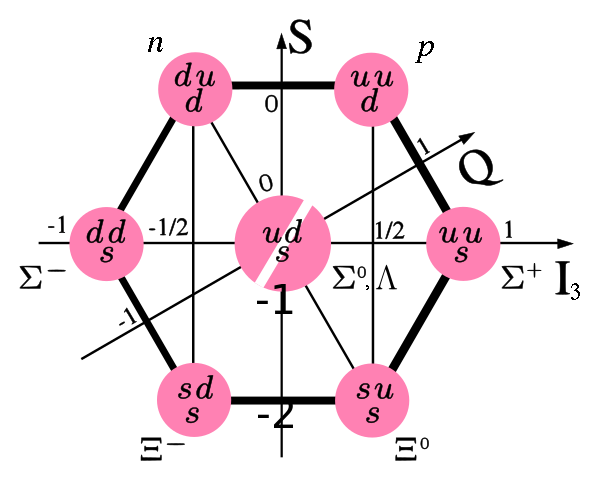
\includegraphics[scale=0.4]{Baryon-octet.png}
	\caption{Baryon--Oktett}
\end{figure}
Mit $u$ und $d$ lassen sich das Proton $uud$ und das Neutron $udd$ bilden. Die Kombinationen $uuu$ und $ddd$ sind aufgrund des Pauli--Prinzipes verboten. 

Die Iso--Spins der beiden koppeln jeweils zu $\pm \nicefrac{1}{2}$, da $u$ den Iso--Spin $I_3 = \nicefrac{1}{2}$ und $d$ den Iso--Spin $I_3 = -\nicefrac{1}{2}$ besitzten. 

\subsection{Das Baryon--Dekuplett $\lp J=\nicefrac{3}{2}\rp$}
Lässt sich analog zum Oktett erklären, allerdings sind nun auch symmetrische Quark--Kombinationen möglich, z.B. $\Delta^{++}$ mit der Kombination $uuu$. 
\begin{figure}[H]
	\centering
	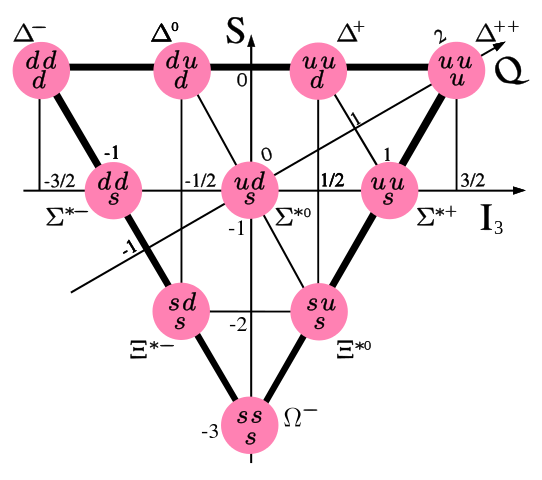
\includegraphics[scale=0.4]{Baryon-decuplet.png}
	\caption{Baryon--Dekuplett}
\end{figure}

Die Wellenfunktion eines Baryons hat Anteile im Orts--, Spin--, und Iso--Spinraum:
\begin{itemize}
	\item Ortswellenfunktion ist für $\Delta^{++}$ symmetrisch, da die 3 up--Quarks ununterscheidbar sind
	\item Da alle 3 Spins zu $\nicefrac{3}{2}$ koppeln, sind auch diese symmetrisch
	\item Analog gilt dies für die Iso--Spin--Wellenfunktion
	\item[$\rightarrow$] Die Gesamtwellenfunktion ist also symmetrisch
\end{itemize}
Fermionen müssen aber \textbf{anti}symmetrische Wellenfunktionen haben! Daher muss für Quarks noch eine weitere Quantenzahl postuliert werden; die \textbf{Farbe}.

Konstruktion von 3 Farben:
\begin{equation}
	\frac{1}{\sqrt{6}} \sum_{i,j,k} \varepsilon_{ijk} u_i u_j u_k
\end{equation}
Theoretische Vorhersagen unter Berücksichtigung der Farbladungen beschreiben die experimentellen Ergebnisse sehr genau. Die theoretischen Vorhersagen stimmen über 6 Zehnerpotenzen min den experimentellen Befundnissen überein. 

\section{Erschließung der Farbladung}
Nun wollen wir die Farbladung etwas genauer betrachten.

Baryonen besitzen 3 Valenzquarks und Gesamtdrehimpuls $\nicefrac{1}{2}$ oder $\nicefrac{3}{2}$. Die Gesamtwellenfunktion setzt sich zusammen aus:
\begin{equation}
	\psi_\text{ges}(1,2,3) =\underset{\text{räumlich}}{\psi_r(1,2,3)} \cdot \underset{\text{Spin}}{\chi_s (1,2,3)} \cdot \underset{\text{Flavour}}{\varphi_f (1,2,3)}
\end{equation}
Wie vorher schon genannt, können wir dennoch Baryonen beobachten, die aus der $uuu$--Kombination bestehen. Also $\exists$ Baryon $(uuu)$ mit Spin $S=\nicefrac{3}{2}$ und $L=0$ $\left[ \Delta^{++} (1232) \right]$.

Dies ergibt aber eine symmetrische Wellenfunktion! Es muss also noch einen Wellenfunktionsanteil geben, sodass die Gesamtwellenfunktion antisymmetrisch ist. Dazu führen wir den Farbladungsanteil $\varphi_c$ ein. 
\begin{equation}
	\varphi_c = \frac{1}{\sqrt{6}} \sum_{r,g,b} \varepsilon_{rgb} u_r u_g u_b
\end{equation}
\subsection{Anzahl der Farben}
\begin{figure}[H]
	\centering
	\feynmandiagram [horizontal=a to b] {
		i1 [particle=$e^-$] -- [fermion] a -- [fermion] i2 [particle=$e^+$],
		a -- [photon, edge label=$\sqrt{\alpha} \qquad \sqrt{q_f^2 \alpha}$] b,
		f1 [particle=$F$]-- [anti fermion] b -- [anti fermion] f2 [particle=$\ol{F}$]
	};
	\caption{Die rechte Seite des Feynman--Diagramms stellt die Hadronisierung dar. Hierbei sind $F,\ \ol{F}$ beliebige Quarks. $q_f$ ist die elektrische Ladung des Flavours f}
\end{figure}
Für Myonenerzeugung ist $q_\mu = \pm 1$. Somit erhalten wir
\begin{equation}
	\sigma\lp e^+ e^- \rightarrow \mu^+ \mu^- \rp = \frac{4\pi \alpha^2 (\hslash c)^2}{3S}
\end{equation}
wobei hier $\sqrt{S}=q^2$ und q der Vierer--Impulsübertrag ist.

Also gilt für $u$--Quarks
\begin{equation}
	\sigma \lp e^+ e^- \rightarrow uu \rp = \sigma \lp e^+ e^- \rightarrow u \ol{u} \rp \cdot q_u^2 \cdot N_{\text{Farbe}}
\end{equation}
womit wir die Größe $R$ definieren können:
\begin{equation}
	R:= \frac{\sigma \lp e^+ e^- \rightarrow \text{Hadronen} \rp}{\sigma \lp e^+ e^- \rightarrow u \ol{u} \rp} = N_{\text{Farbe}} \sum_f q_f^2
\end{equation}
$N_{\text{Farbe}}$ wird auch die \textbf{Multiplizität} der Farbe genannt.
\begin{table}[h]
	\centering
	$
	\begin{array}{rcl}
		\sqrt{S} & \textbf{Schwelle} & R \\ \hline
		\leq 2\cdot 494 \si{MeV} & K^+ K^- & 3\lp \nicefrac{4}{9} + \nicefrac{1}{3} \rp = \nicefrac{5}{2} \\ 
		\text{bis } 3729 \si{MeV} & D \ol{D} \text{ (aus c--Quark)} & 2 \\ 
		\text{bis } 10.6 \si{GeV} & B\ol{B} \text{ (b--Quark)} & \nicefrac{10}{3} \\ 
		\text{oberhalb} & \text{(alle außer t--Quark (erst ab $\approx 30 \si{GeV}$))} & \nicefrac{11}{3}
	\end{array} 
	$
\end{table}

\section{Jets}
Woher wissen wir nun, dass es Gluonen gibt?
Quarks können aufgrund der Confinement--Hypothese nicht allein existieren. Da Quarks und Gluonen in gebundenen Zuständen existieren, ist es sehr schwer, Gluonen nachzuweisen. Versucht man, zwei Quarks zu trennen, wird ihnen dabei so viel Energie zugeführt, dass sich daraus sofort ein neues Quark--Antiquark--Paar bildet, bevor sich die ursprünglichen Quarks trennen lassen. Bei einer $e^-$--$e^+$--Kollision entsteht genug Energie, sodass dieser Prozess gleich mehrfach abläuft: 
\begin{figure}[H]
	\centering
	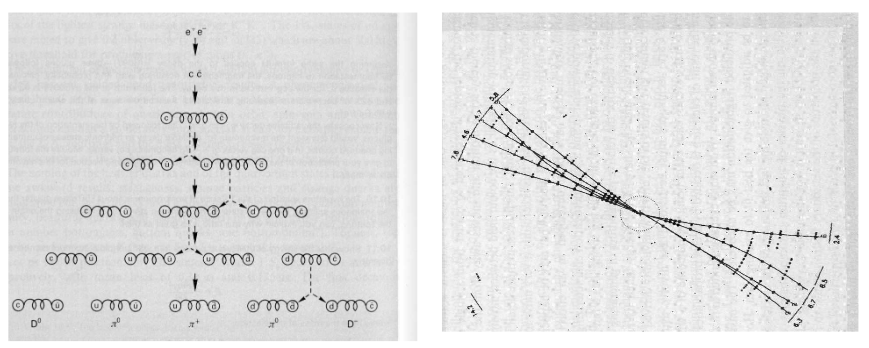
\includegraphics[scale=0.4]{jets_ee-kollision.png}
	\caption{Links: Prinzip des Prozesses. Rechts: Hadronen--Jets im Experiment}
\end{figure}
Da auf diese Art viele Hadronen in zwei Vorzugsrichtungen ''sprengen'', nennt man dies \textbf{Hadronen--Jets}. Ein typisches 2--Jet--Ereignis ist $e^- + e^+ \rightarrow q + \ol{q}$

Man ging davon aus, dass ähnlich wie bei der Elektronenbremsstrahlung bei genügend hoher Energie Gluonen von den Quarks abgestrahlt werden können, welches ebenfalls einen Jet erzeugt. Somit müsste man manchmal auch einen dritten Jet beobachten, was 1979 am DESY festgestellt wurde. Diese 3--Jet--Ereignisse treten etwa 10 mal seltener auf, als die 2--Jet--Ereignisse.

\section{Trivia}
Neben Mesonen und Baryonen gibt es mehr Hadronen:
\begin{itemize}
	\item Tetraquarks: Hypothetische Teilchen aus 2 Quarks und 2 Antiquarks
	\item Pentaquarks: Teilchen aus 3 Quarks und einem Quark--Antiquark--Paar. (2015 erstmals am LHC gemessen!)
	\item Gluebälle: Hypothetische Teilchen aus null Valenzquarks, sondern nur Gluonen und Seequarks.
	\item Quark--Gluonen--Plasma: besteht aus vielen Quarks, die Dynamik ähnelt einer Flüssigkeit. Durch hohe Dichte ist die Confinement--Hypothese quasi aufgehoben. Allerdings fehlt eine genaue theoretische Beschreibung bisher leider. 
\end{itemize}
\end{document}